\documentclass{article}
\usepackage[utf8]{inputenc}
\usepackage{amsmath,amssymb,amsthm,mathrsfs,graphicx}

\title{HW5}
\author{Ry Wiese\\wiese176@umn.edu}
\date{October 20, 2019}

\begin{document}

\maketitle

\section{Problem 1}

\subsection{Part 1}

\[
\begin{array}{rrcl}
 \min & 4y_1 + 7y_2  &      &   \\
 \mbox{s.t.}  &  2y_1 + y_2  & \ge & 5~; \\
              &  3y_1 + 2y_2 & \ge & 2~; \\
              &  y_1 + 3y_2 & \ge & 5~; \\
     &   \mathbf{y}  & \geq & \mathbf{0}~.
\end{array}
\]

\subsection{Part 2}

\begin{figure}[h] % "h" is where to place, h=here, t=top, b=bottom
  \centering
  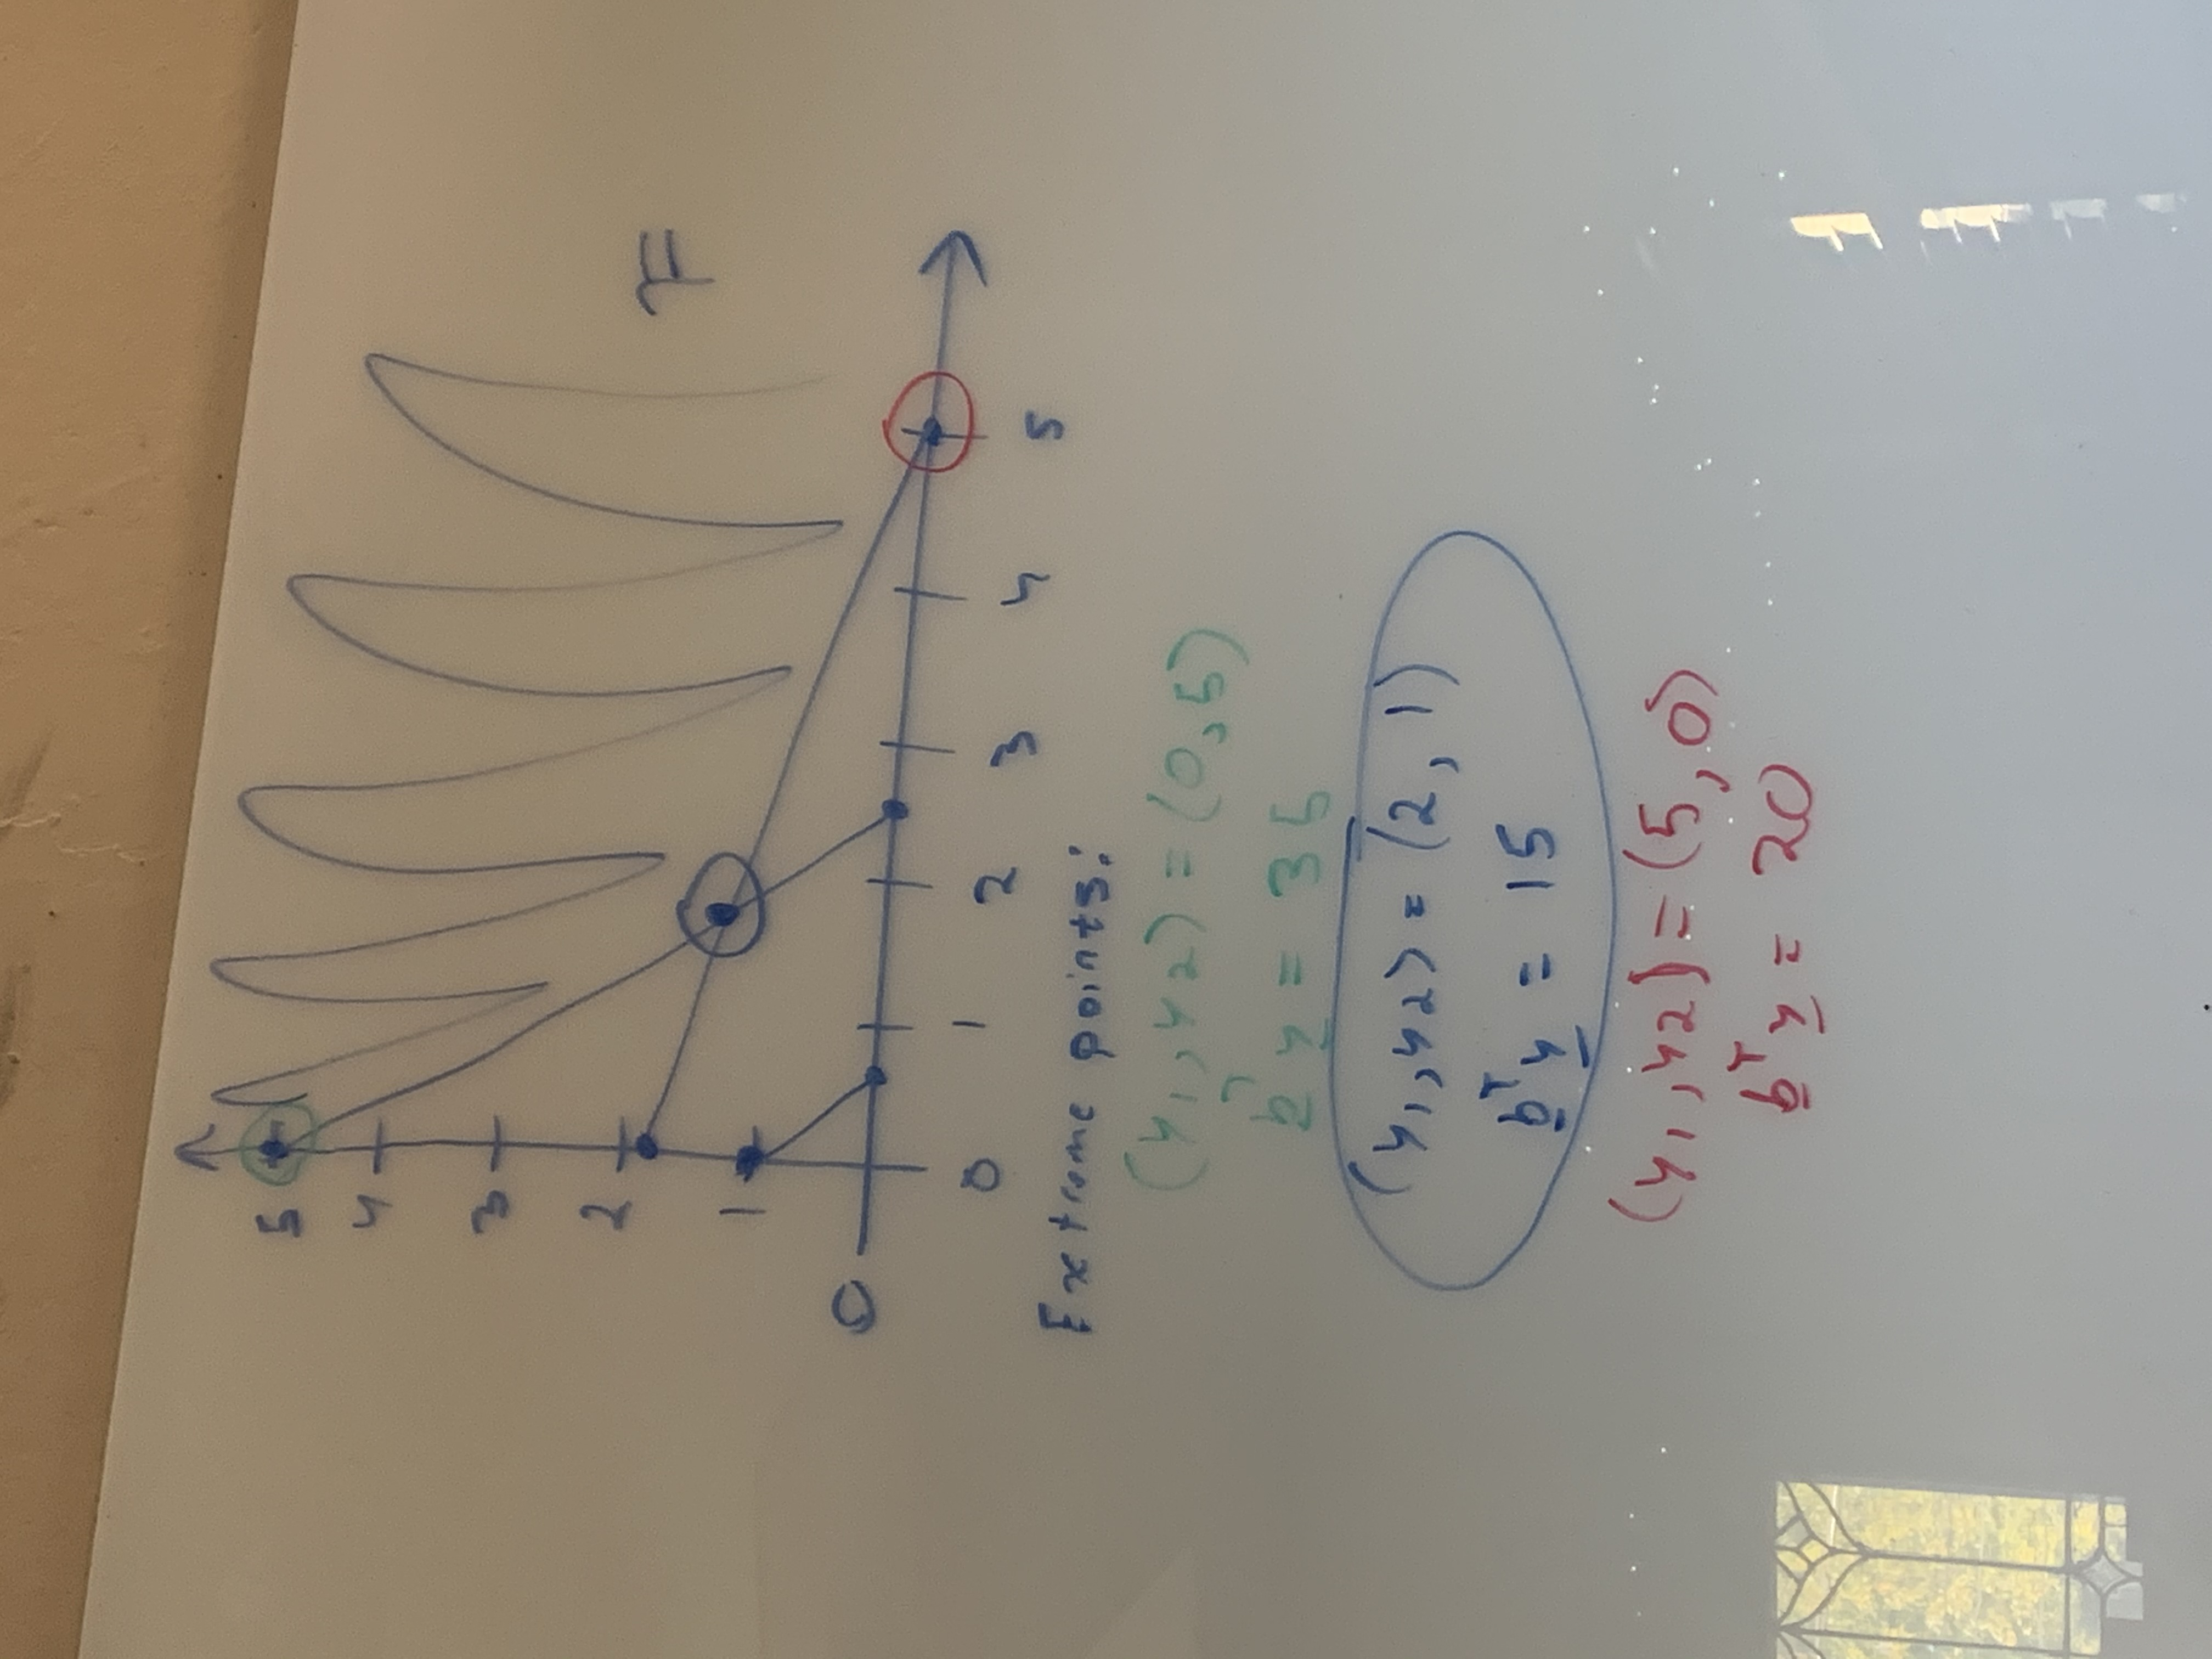
\includegraphics[angle=270,totalheight=80mm]{P1.jpg}
  \caption{Graph of the dual problem.}
  \label{fig:tabl}
\end{figure}

The optimal solution of the dual problem is $(y_1, y_2) = (2, 1)$, which has an optimal value of 15.

\subsection{Part 3}

When $j=1$,
$$x_1(2y_1 + y_2 - 5) = 0$$
$$x_1(2(2) + (1) - 5) = 0$$
$$0 = 0.$$

When $j=2$,
$$x_2(3y_1 + 2y_2 - 2) = 0$$
$$x_2(3(2) + 2(1) - 2) = 0$$
$$6x_2 = 0$$
$$x_2 = 0.$$


When $j=3$,
$$x_3(y_1 + 3y_2 - 5) = 0$$
$$x_3((2) + 3(1) - 5) = 0$$
$$0 = 0.$$

At this point, we know that $x_2 = 0$.\\

When $i=1$,
$$y_1(2x_1 + 3x_2 + x_3 - 4) = 0$$
$$y_1(2x_1 + x_3 - 4) = 0$$
$$2(2x_1 + x_3 - 4) = 0$$
$$4x_1 + 2x_3 = 8.$$

When $i=2$,
$$y_2(x_1 + 2x_2 + 3x_3 - 7) = 0$$
$$y_2(x_1 + 3x_3 - 7) = 0$$
$$x_1 + 3x_3 - 7 = 0$$
$$x_1 + 3x_3 = 7.$$

Solving $4x_1 + 2x_3 = 8$ and $x_1 + 3x_3 = 7$ gives us $x_1 = 1$ and $x_3 = 2$, with $x_2 = 0$. It can be verified that $\mathbf{c}^T\mathbf{x} = 15$ in the primal problem.

\section{Problem 2}

\subsection{Part 1}
Process 1 generates a profit of $4(38) + 3(33) - 51 = 200$. Process 2 generates a profit of $(38) + (33) - 11 = 60$. Process 3 generates a profit of $3(38) + 4(33) - 40 = 206$. Thus we can formulate the LP as 
\[
\begin{array}{rrcl}
  - \min & \mathbf{c}^T \mathbf{x}  &      &   \\
 \mbox{s.t.}  &  A\mathbf{x}  &   =  & \mathbf{b}~; \\
      &   \mathbf{x}  & \geq & \mathbf{0}~
\end{array}
\]
where
\[
\mathbf{b} = 
\left(
  \begin{array}{c}
    8000 \\
    5000 \\
  \end{array}
\right), 
~
\mathbf{c} = 
\left(
  \begin{array}{c}
    -200 \\
    -60 \\
    -206 \\
    0 \\
    0 \\
  \end{array}
\right), 
~
A = 
\left(
  \begin{array}{ccccc}
    3 & 1 & 5 & 1 & 0 \\
    5 & 1 & 3 & 0 & 1 \\
  \end{array}
\right).
\]

$\mathbf{Step~1}$:\\
BFS: $\mathbf{x}_B = 
\left(
    \begin{array}{c}
        1000\\
        0\\
        0\\
        5000\\
        0\\
    \end{array}
\right)$\\
Objective value: $\mathbf{c}^T \mathbf{x} = -200000$\\
Reduced costs: $\mathbf{\bar{c}} =  
\left(
    \begin{array}{c}
        0\\
        -20\\
        -86\\
        0\\
        40\\
    \end{array}
\right)$\\
Index to enter: 2\\
Basic direction: $\mathbf{d} = \left(
    \begin{array}{c}
        -.2\\
        1\\
        0\\
        -.4\\
        0\\
    \end{array}
\right)$\\
Index to exit: 1\\
\\
\\
$\mathbf{Step~2}$:\\
BFS: $\mathbf{x}_B = 
\left(
    \begin{array}{c}
        0\\
        5000\\
        0\\
        3000\\
        0\\
    \end{array}
\right)$\\
Objective value: $\mathbf{c}^T \mathbf{x} = -300000$\\
Reduced costs: $\mathbf{\bar{c}} =  
\left(
    \begin{array}{c}
        100\\
        0\\
        -26\\
        0\\
        60\\
    \end{array}
\right)$\\
Index to enter: 3\\
Basic direction: $\mathbf{d} = \left(
    \begin{array}{c}
        0\\
        -3\\
        1\\
        -2\\
        0\\
    \end{array}
\right)$\\
Index to exit: 4\\
\\
\\
$\mathbf{Step~3}$:\\
BFS: $\mathbf{x}_B = 
\left(
    \begin{array}{c}
        0\\
        500\\
        1500\\
        0\\
        0\\
    \end{array}
\right)$\\
Objective value: $\mathbf{c}^T \mathbf{x} = -339000$\\
Reduced costs: $\mathbf{\bar{c}} =  
\left(
    \begin{array}{c}
        74\\
        0\\
        0\\
        13\\
        47\\
    \end{array}
\right)$\\
\\
We are now done. The optimal solution is $\mathbf{x}_B = 
\left(
    \begin{array}{c}
        0\\
        500\\
        1500\\
        0\\
        0\\
    \end{array}
\right)$ with an objective value of \$339000.

\subsection{Part 2}

Let $\mathbf{c}' = \mathbf{c} + \Delta \left( \begin{array}{c} -4\\-1\\-3\\0\\0 \end{array} \right)$ denote the new cost vector associated with the changed price. In order for $B = \{2, 3\}$ to remain the optimal basis, we must insist that $\bar{\mathbf{c}}_N = \mathbf{c}'_N - (A_B^{-1}A_N)^T \mathbf{c}'_B \ge \mathbf{0}$.\\
$A_B = \left( \begin{array}{cc} 1 & 5\\ 1 & 3\\ \end{array} \right)$ and $A_N = \left( \begin{array}{ccc} 3 & 1 & 0\\ 5 & 0 & 1\\ \end{array} \right)$.\\
$\bar{\mathbf{c}}_N = \mathbf{c}'_N - (A_B^{-1}A_N)^T \mathbf{c}'_B = \left( \begin{array}{c} -200\\-0\\-0\\ \end{array} \right) + \Delta \left( \begin{array}{c} -4\\0\\0\\ \end{array} \right) - (\left( \begin{array}{cc} 1 & 5\\ 1 & 3\\ \end{array} \right)^{-1} \left( \begin{array}{ccc} 3 & 1 & 0\\ 5 & 0 & 1\\ \end{array} \right))^T (\left( \begin{array}{c} -60\\-206\\ \end{array} \right) + \Delta \left( \begin{array}{c} -1\\-3\\ \end{array} \right)) = \left( \begin{array}{c} 74 + \Delta\\ 13\\ 47 + \Delta \end{array} \right) \ge \mathbf{0}$.\\
Thus the optimal solution will change only if $\Delta > 47$.

\subsection{Part 3}

The optimal solution will be the same as in Part 1. The optimal solution of $x_2 = 500$ and $x_3 = 1500$ only produces $3x_2 + 5x_3 = 9000 \le 10000$, so all constraints are still satisfied.

\section{Problem 3}

\subsection{Part 1}

If $x_1$ is the number of units of special risk insurance, $x_2$ is the number of units of mortgage insurance, and $x_3$ is the number of units of long term care insurance, then the LP can be formulated as follows:
\[
\begin{array}{rrcl}
  \max & \mathbf{c}^T \mathbf{x}\\
 \mbox{s.t.}  &  A \mathbf{x}  & \le & \mathbf{b}~\\
 & \mathbf{x} & \ge & \mathbf{0}.
\end{array}
\]
where $\mathbf{c} = \left( \begin{array}{c} 500\\ 250\\ 600\\ \end{array} \right)$, $\mathbf{b} = \left( \begin{array}{c} 240\\ 150\\ 180\\ \end{array} \right)$, and $A = \left( \begin{array}{ccc} 2 & 1 & 1\\ 3 & 1 & 2\\ 1 & 2 & 4\\ \end{array} \right)$.

\subsection{Part 2}

The dual problem can be written as
\[
\begin{array}{rrcl}
  \min & \mathbf{b}^T \mathbf{y}\\
 \mbox{s.t.}  &  A^T \mathbf{y}  & \ge & \mathbf{c}~\\
 & \mathbf{y} & \ge & \mathbf{0}.
\end{array}
\]
Solving the dual problem gives a solution of $\mathbf{y} = \left( \begin{array}{c} 0\\ 140\\ 80\\ \end{array} \right).$ Then, we can list out all of the complementarity conditions in terms of $\mathbf{y}$.
$$x_1(2y_1 + 3y_2 + y_3 - 500) = x_1(3 \cdot 140 + 80 - 500) = 0 \cdot x_1 = 0$$
$$x_2(y_1 + y_2 + 2y_3 - 250) = x_2(140 + 2 \cdot 80 - 250) = 50x_2 = 0$$
$$x_3(y_1 + 2y_2 + 4y_3 - 600) = x_1(2 \cdot 140 + 4 \cdot 80 - 600) = 0 \cdot x_3 = 0$$
The first and third of the above equations are true for all values of $x_1$ and $x_3$, but the second equation is only true for $x_2 = 0$. Thus no mortgage insurance is sold.

\subsection{Part 3}

In order for $B$ to be the optimal basis, $\mathbf{x}_B' = A_B^{-1}(\mathbf{b} + \Delta \mathbf{e}_3) = \mathbf{x}_B + \Delta A_B^{-1} \mathbf{e}_3 = \left( \begin{array}{c} 24\\ 39\\ 153\\ \end{array} \right) + \Delta \left( \begin{array}{c} -.2\\ .3\\ .1\\ \end{array} \right) \ge \mathbf{0}$. Thus $\Delta \le \frac{-24}{-.2} = 120$, $\Delta \ge \frac{-39}{.3} = -130$, and $\Delta \ge \frac{-153}{.1} = -1530$. Since $\mathbf{b} \ge \mathbf{0}, -180 \le \Delta \le 120$.

\subsection{Part 4}

In order for $B$ to be the optimal basis,\\ $\bar{\mathbf{c}}_N = \mathbf{c}_N - (A_B^{-1}A_N)^T(\mathbf{c}_B + \Delta \mathbf{e}_1) = \left( \begin{array}{c} -250\\ 0\\ 0\\ \end{array} \right) - (\left( \begin{array}{ccc} 0 & .4 & -.2\\ 0 & -.1 & .3\\ 1 & -.7 & .1\\ \end{array} \right) \left( \begin{array}{ccc} 1 & 0 & 0\\ 1 & 1 & 0\\ 2 & 0 & 1\\ \end{array} \right))^T \left( \begin{array}{c} -500 + \Delta \\ -600\\ 0\\ \end{array} \right) = \left( \begin{array}{c} 3290\\ 140 - .4 \Delta \\ 1700 + .2 \Delta \\ \end{array} \right)\ge \mathbf{0}$.\\
Thus $\Delta \le \frac{140}{.4} = 350$ and $\Delta \ge \frac{1700}{-.2} = -8500$. 

\section{Problem 4}

\begin{proof}

Let $P$ be defined as
\[
\begin{array}{rrcl}
 \max & 0\\
 \mbox{s.t.}  &  A \mathbf{x}  & = & \mathbf{b}~.\\
\end{array}
\]
Clearly, $P$ has a solution iff system 1 has a solution. We can represent $dual(P)$ as
\[
\begin{array}{rrcl}
 \min & \mathbf{b}^T \mathbf{y}\\
 \mbox{s.t.}  &  A^T \mathbf{y}  & = & \mathbf{0}~ \\
 &   \mathbf{y}  & \ge & \mathbf{0}~.
\end{array}
\]

We start by showing that no more than one of the two systems can have a solution. We do this by showing that if system 2 has a solution, then system 1 cannot. Assume that $\hat{\mathbf{y}}$ is a solution to system 2. Then, for any $\lambda > 0$, $A^T (\lambda \hat{\mathbf{y}}) = ((\lambda \hat{\mathbf{y}})^TA)^T = \lambda (\hat{\mathbf{y}}^T A)^T = \lambda \mathbf{0} = \mathbf{0}$. Since $\hat{\mathbf{y}} \ge \mathbf{0}$ and $\lambda > 0$, $\lambda \hat{\mathbf{y}} \ge \mathbf{0}$. Thus $\lambda \hat{\mathbf{y}}$ is a feasible solution to $dual(P)$. Since $\mathbf{b}^T \hat{\mathbf{y}} < 0$ and $\lambda > 0$, $\mathbf{b}^T (\lambda \hat{\mathbf{y}}) = \lambda \mathbf{b}^T \hat{\mathbf{y}} < 0$. Thus, $\mathbf{b}^T (\lambda \hat{\mathbf{y}})$ has no minimum value, since $\lambda$ can be arbitrarily large, so $dual(P)$ is unbounded and therefore $P$ is infeasible. Thus system 1 does not have a solution.

Now we show that at least one of the two systems must have a solution. We do this by showing that if system 2 is infeasible, system 1 must be feasible. Assume that system 2 is infeasible. Since $A^T \mathbf{0} = 0$ and $\mathbf{0} \ge \mathbf{0}$, $\mathbf{0} \in \mathcal{F}_{dual(P)} \ne \emptyset$. $dual(P)$ is not infeasible. Then, let $\hat{\mathbf{y}} \in \mathcal{F}_{dual(P)}$ be any feasible solution to $dual(P)$. $A^T \hat{\mathbf{y}} = \mathbf{0}$ and $\hat{\mathbf{y}} \ge \mathbf{0}$. Since system 2 is not feasible, it must be that $\mathbf{b}^T \hat{\mathbf{y}} \ge 0$. Then, $\min \{\mathbf{y} \in \mathbb{R}^n ~|~ \mathbf{y} \in \mathcal{F}_{dual(P)}\} \ge 0$, therefore $dual(P)$ is not unbounded. $dual(P)$ must have an optimal solution, and therefore $P$ has an optimal solution as well. So system 1 has a solution.

\end{proof}

\end{document}
